
\begin{htmlonly}


\usepackage{html, htmllist}
\usepackage{longtable}

\bodytext{bgcolor="#ffffff" link="#0033cc" vlink="#0033cc"}

%%%==================================================	
%%%==================================================	

% #1  mark defined by \label
% #2  a linktext 
% #3  a html link 
\newcommand{covlink}[3]{\htmladdnormallink{#2}{#3} \latex{(\ref{#1})} }


\newenvironment{covimg}[4]%
{
 \begin{figure}[htp]
  \begin{center}
   \latexonly
      \includegraphics[scale=#4]{#1/pict/#2}
   \endlatexonly  
   \html{\htmladdimg[align="center"]{pict/#2.png}}
   \caption{#3}
  \end{center}
 \end{figure} 
}{} 

\newenvironment{covimg2}[3]%
{ 
 \begin{figure}[htp]
  \begin{center}
     \latexonly
       \includegraphics[scale=#3]{#1/pict/#2}   
     \endlatexonly
     \html{\htmladdimg[align="center"]{pict/#2.png}}
  \end{center}
 \end{figure} 
}{}

\definecolor{output}{rgb}{0.,0.,1.}
\definecolor{depend}{rgb}{1.,0.65,0.}
\definecolor{required}{rgb}{0.58,0.,0.83}
\definecolor{optional}{rgb}{0.,0.39,0.}

\newcommand{\addimage}[1] {\html{\htmladdimg{pict/#1.png}}}

\newcommand{\addpict}[4] {\latexonly
	     \begin{figure}[!htbp]
			  \begin{center}
   	 		  \includegraphics[scale=#1]{#2}
   	 		  \caption{#3}
		 		  \label{#4}
			  \end{center}
	 		\end{figure}
	     \endlatexonly}



\newcommand{\mapeditor}{\textbf{Map Editor}}
\newcommand{\covise}{\textbf{COVISE}}


\end{htmlonly}


%=============================================================
\startdocument
\chapter{COVER}
\label{COVER}
%=============================================================

COVER (COvise Virtual Environment Renderer) is a COVISE renderer module
with support for Virtual Reality (VR) input devices, backprojection displays,
and intuitive interaction. 
COVER can also be started independendly of COVISE and just be used as a virtual
reality viewer for 3D geometry.

To start COVER within COVISE, select the module COVER in the module list
under the category Renderer.

To start COVER as a 3D viewer, type in 
\begin{verbatim}
    cover <filename>
\end{verbatim}

{\it Note: Please make sure to set the variable DISPLAY in your environment before starting
COVER!}

COVER is based on Performer, a high level 3D graphics library from
SGI, providing high speed rendering, multi-processing, multi-pipe,
scene graph, loaders for 3D database formats...
Performer is available for IRIX and Linux platforms.

This chapter about COVER describes the {\large {\bf COVER User Interface}} and 
has the two sections:

\begin{itemize}
\item \html{\htmladdnormallink{Interaction in COVER}{Interaction.html}}\latex{{\bf Interaction in COVER}
(\ref{label_chapter_interaction})}:
This section describes how to use COVER. It explains the entries in the 3D menu and the corresponding interaction techniques. 
\item  \html{\htmladdnormallink{PlugIns}{Plug_Ins.html}} \latex{{\bf PlugIns}
(\ref{Plug_Ins})}:
This section describes the plugins "Probe" and "Viewpoints".
\end{itemize}

For configuration of displays and input devices see the separate document \newline

 {\it COVER Installation and Configuration}\newline

with the sections

\begin{itemize}
\item {\bf Graphics Board and Display}: 
This section explains which types of Virtual Environments are supported and how to configure COVER and your graphics workstation for this Virtual Environment.
\item {\bf Input Devices}: This section explains which types of Virtual Environments are supported and how
to configure COVER and your graphics workstation for this Virtual Environment.
\end{itemize}

%\item[\html{\htmladdnormallink{Graphics Board and Display}{Graphics_Board_Display.html}}
%\latex{{Graphics Board and Display } (\ref{label_chapter_display})}]
%This section explains which
%types of Virtual Environments are supported and how
%to configure COVER and your graphics workstation for this Virtual Environment.

%\item[\html{\htmladdnormallink{Input Devices}{Input_Devices.html}}
%\latex{{Input Devices} (\ref{label_chapter_input})}]
%This section explains which
%3D input and tracking devices are supported and how to configure 
%COVER for your specific devices.

%\newpage
%\input cover/display/display 
%\newpage
%\input cover/input/input


\section{Interaction}
\label{label_chapter_interaction}

COVER can be used either as a viewer for 3D scenes or as a renderer
module in COVISE.

As a 3D viewer COVER supports all 3D file formats which are also supported by the 
graphics library OpenGL Performer and additionally vrml files with 
sound and interaction. To load a specific file call COVER with the file 
name as parameter:
\begin{samepage}
\begin{verbatim}
    cover <filename>
\end{verbatim}
\end{samepage}


As a COVISE renderer module COVER is started through the Mapditor. Select the category renderer
and drag the module COVER to the map area. You can now connect all modules
to COVER which generate geometric primitives like lines, triangle strips, 
polygons or points with colors, normals and textures.

\begin{covimg}{cover}{renderer_start}{Starting COVER as COVISE Renderer Module}{0.7}\end{covimg}

If you have a full COVISE installation you will recognize that there
are two COVERs: one called COVER and one called COVER\_VRML. Only the
second one supports vrml files with sound and interaction. As you don't
need this functionality for most COVISE visualisations, a smaller 
version without vrml support, named COVER, is provided, too.

\label{label_tracking_3dpointer}
\subsection{Headtracking and 3D Pointer}
In COVER the user can freely move in the virtual scene  
and manipulate it with a 3D input device.

The movement of the user is measured with a sensor 
mounted at the glasses. With the measured position and orientation an 
appropriate view on the scene is computed. This is called head tracking.
Currently only one user can be tracked. Other users don't have the correct 
view of the scene and therefore they have the impression that all objects 
are slightly distorted. This effect is minimized if they try to stand close 
to the user with the tracked glasses and try to look into the same 
direction as the one with the tracked glasses. 

The location and orientation of the 3D input device, which the user
holds in his hand, is measured through a sensor in the input device.
The input device usually has one two three buttons. One button is 
used to indicate a selection. On a three button device the other two buttons
are used to switch the navigation mode without using the 3D menu.

With the virtual laser beam which seems to come out of the 3D input device also
remote objects can be reached, for example buttons in the 3D menu.

\begin{covimg}{cover}{menu_selection}{Selecting a menu entry with the laser beam}{0.7}\end{covimg}

\subsubsection{Using COVER with the mouse}
COVER can also be used with the mouse. The viewer position is then fixed to
the position defined in covise.config:
\begin{samepage}
\begin{verbatim}
COVERConfig
{
    ...
    TRACKING_SYSTEM MOUSE
    VIEWER_POSITION  <x> <y> <z>
    ...
}
\end{verbatim}
\end{samepage}



The interaction possibilities with the menu and the 3D scene are described
in the following chapters.

\label{label_chapter_stereo}
\subsection{Stereo Viewing}

For the stereo projection two images are generated, one with the perspective
of the right eye and one with the perspective of the left eye. The stereo
glasses show only the appropriate image to each eye. Like stereo viewing
in reality the brain forms a 3D impression of the scene.

And similar to reality objects which are very close to the users head
are seens twice because the two images can't be fused any more, objects
which are very far don't appear to be three dimensional but flat.
Therefore the optimal location of obejcts for stereo viewing are not too
near and not too far. 

If the scene size fits into the virtual reality
environment, the best position is near the front screen, optimally one part
of the scene is in front of the screen and the other part behind. 
For many technical visualisations for example flow visualisation of
the air around a car the scene can be scaled so that it fits into the
virtual environment (see chapter xy view all).

Larges scenes like landscapes are best viewed on large screens.
If the scene is larger than the screens, but the screen is so small that it 
is inside the users field of view the stereo impression can get lost, 
when the object is located in  front of the screen. 
This happens because the human brain is so used to the fact that in reality
objects partly covered by something are behind that it can't form a stereo 
impression if a virtual scene is cut by the frame of the screen. 
Therefore for large scenes and small screens  the best position is behind 
the screen and the screens is like a window to the outside.

\label{label_chapter_3dmenu}

\subsection{3D Menu}

The navigation mode, viewing options, and manipulation modes are
selected through a 3D menue, called the Pinboard. You select a menu entry
by pointing to the button with the laser beam and pressing the 
button of the 3D input device. If the pinboard is used with a mouse
simply bring the mouse pointer over the menu entry and click a button.

The COVER Pinboard can be re-positioned in the VE by pointing to the title bar
and pressing the button of the 3D input device.If you have a 3-button device
and select it the left button, the menu is rotated around it's z axis so it 
always faces the viewer (billboard mode). Selected with the right button, it moves as if it's
mouned at the laser beam. Selected with the middle mouse button
it changes it's size according to the rotation of the users arm. 

The same applies for mouse input: left mouse button moves the menu in a 
way that it faces the viewer, right mouse button moves the menu with the
mouse pointer. The orientation is defined through a line from the viewer
to the mouse so it seems to face the viewer, too. Middle mouse button
scales the menu, movements up and down make the menu larger and smaller. 

For one-button devices the billboard mode and the scaling is not supported.


\begin{covimg}{cover}{drag}{Menu Positioning}{0.5}\end{covimg}

The initial position, orientation, size, layout of the menu and the start 
values of toggleand group buttons can be specified in the file covise.config
(see configuration in cover installation guide).

\subsubsection{Menu Button Types}

In the 3D menu there are three different types of buttons.

\paragraph{Simple Buttons} with only a label execute a certain function once, for example
if you press the "view all"  button , the scene is scaled once so that 
it fits onto the screen.

\paragraph{Toggle buttons} 
\latexonly

\includegraphics[scale=0.5]{cover/pict/toggle_button_icon} 
\endlatexonly
\html{\htmladdimg[ALIGN=TOP]{pict/toggle_button_icon.png}}
switch between two states, for example you can
switch headtracking on or off.


\paragraph{Radio buttons} 
\latexonly

\includegraphics[scale=0.5]{cover/pict/radio_button_icon} 
\endlatexonly
\html{\htmladdimg[SCALE=0.5 ALIGN=TOP]{pict/radio_button_icon.png}}
select one function in a group of functions.
All navigation functions are in such a button group, if you you have 
"move world" on and then switch to "scale world" the "move world" button 
is switched off. 
All collaborative working modes are also in a separate button group.
Group buttons can be spread across the menu and the submenus.

\paragraph{Slider buttons} 
\latexonly
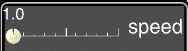
\includegraphics[scale=0.5]{cover/pict/slider_button} 
\endlatexonly
\html{\htmladdimg[ALIGN=TOP]{pict/slider_button.png}}
are used to select a numerical value between a minimum
and a maximum value. The "drive speed" button is such a slider button.
Currently only floating value slider buttons are implemented.

\paragraph{Submenu buttons} open a new menu. The submenu can be selected
and dragged like the pinboard.

\begin{covimg}{cover}{submenu_button}{Submenu Button}{0.5}\end{covimg}


	
\subsection{Navigation Modes}
With the functions XFORM, SCALE, FLY, DRIVE, WALK
the user navigates through the scene. These functions are grouped into
a radio button group, therefore only one navigation mode can be active.

\subsubsection{Move World (XFORM)}
\latexonly
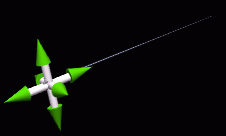
\includegraphics[scale=0.5]{cover/pict/xform} 
\endlatexonly
\html{\htmladdimg[ALIGN=TOP]{pict/xform.png}}

In XFORM mode (XFORM stands for transform) the whole scene 
(besides the coordinate axis and the pinboard) can be moved. 
The default button label is "move world" and
the default button location is in the main Pinboard menue. 
The XFORM mode indicated with the above 3D icon.

Only when the button of the 3D input device is pressed, the world
is translated and rotated with the users hand. The translation is relative 
to the point where the button was pressed. The center of rotation is the users
hand. The interaction is stopped when the button is released. For pulling
the whole scene closer to the user you can move the hand away from the body, 
then press the button and move the hand closer too th body, and then relase 
the button. Do this several times if the appropriate position can't be 
reached in one step. 

If the input device is the mouse, the scene is rotated when the left
mouse button is pressed and translated when the middle mouse button
is pressed. In rotate mode, up/down movements rotate around the x axis, 
left/right movements rotate around the z axis. In translate mode, up/down
movements translate into positive and negative z direction, left/right movements 
into positive/negative x axis.
		
\subsubsection{Scale World (SCALE)}
\latexonly
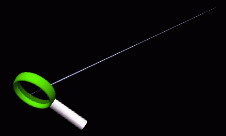
\includegraphics[scale=0.5]{cover/pict/scale} 
\endlatexonly
\html{\htmladdimg[ALIGN=TOP]{pict/scale.png}}

In SCALE mode the whole scene (besides the coordinate axis and the pinboard) 
can be scaled. 
The default button label is "scale world" and
the default button location is in the main Pinboard menue. 
The button belongs to the button group "Navigation".
The SCALE mode indicated with a magnifying class as 3D icon.

When the button of the 3D input device is pressed and the hand is
moved to he right, the world becomes larger, when the hand is moved
to the left, the world becomes smaller. The interaction is stopped when the
button is released.

The same applies for mouse input.
 		
\subsubsection{View All (VIEW\_ALL)}

When the VIEW\_ALL button is pressed, the whole scene 
(besides the coordinate axis and the pinboard) 
is scaled so that it fits into the visible part of the world - 
typically the screen size. 
The default button label is "view all" and
the default button location is in the main Pinboard menue. 
The button is a function button.

The size for the scaling is defined in the file covise.config in 
the section COVERConfig
with the keyword SZENE\_SIZE. It is defined in mm. A 19'' Monitor for
example has 340 x 270 mm, there a good choice would be 270, in a 
CAVE with the wall size 2800 x 2500 mm we would choose 2500.

\begin{samepage}
\begin{verbatim}
COVERConfig
{
    ...
    SCENE_SIZE <size in mm>
    ...
}
\end{verbatim}
\end{samepage}

COVER also supports an "autoscale" mode. In this mode a "view all" is performed
every time a new object is appended to the scene graph. You enable
this mode in the scope COVERConfig with the keyword SCALE\_ALL.
\begin{verbatim}
COVERConfig
{
    ...
    SCALE_ALL <ON or OFF>
    ...
}
\end{verbatim}

		
\subsubsection{Stop Headtracking (FREEZE)}
With FREEZE headtracking is enabled/disabled. 
The default button label is "headtracking" and
the default button location is in the main Pinboard menue. 
The button is a toggle button. The default state is 
OFF, this means headtracking is enabled. 

Freezing the current view can be useful for demonstrations with many 
people, where it is
impossible, that all users move with the demonstrator. Or for taking
pictures or making a video. There you get the best results when the
camera position matches the viewer position. In some configurations
the camera must be in the area where the magnetic tracking system doesn't
deliver correct values. Then you can freeze headtracking at starting time and
specify a viewer position:

\begin{verbatim}
COVERConfig
{
    ...
    FREEZE ON
    VIEWER_POSITION 	0 -3000 500
    ...
}
\end{verbatim}
This means for example the viewpoint is 3 m in negative y direction and
50 cm above the origin in z direction. The Performer coordinate system is
x=RIGHT, z=UP, and Y=into the screen.

		
\subsubsection{FLY}
\latexonly
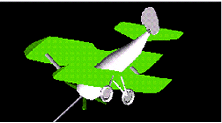
\includegraphics[scale=0.5]{cover/pict/fly} 
\endlatexonly
\html{\htmladdimg[ALIGN=TOP]{pict/fly.png}}

In FLY mode the whole scene (besides the coordinate axis and the pinboard) 
is moved as if the user sits in an airplane. 
The default button label is "fly" and
the default button location is in the "Navigation" submenu. 
The button belongs to the button group "Navigation".
The FLY mode indicated with an airplane as 3D icon.

You start the fly mode by pressing the button of the 3D input device
and then moving the hand into the direction you want to fly.
Moving the hand far away from the point where you pressed the button 
results in faster flying. Moving the hand close to the body behind the point
where you pressed the button, results in flying backwards.
A scale factor for the fly speed can be applied with the slider "SPEED".

Mouse input in fly mode doesn't work.		
\subsubsection{WALK}
\latexonly
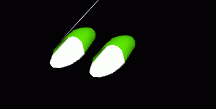
\includegraphics[scale=0.5]{cover/pict/walk} 
\endlatexonly
\html{\htmladdimg[ALIGN=TOP]{pict/walk.png}}

In WALK mode the whole scene (besides the coordinate axis and the pinboard) 
is moved as if the user walks in the scene. 
The default button label is "walk" and
the default button location is in the "Navigation" submenu. 
The button belongs to the button group "Navigation".
The WALK mode is indicated with shoes as 3D icon.

You start the walk mode by pressing the button of the 3D input device
and then moving the hand into the direction you want to walk. COVER
then intersects a line from the feet into the negative z direction (towards the
bottom) with the scene and if close enough, repositions the user on that
point in the scene. 
As the feet are not tracked, the feet position is calculated from the
head position  and the floorHeight and the stepSize. FloorHeight and stepSize
are specified in the section COVERConfig in the file covise.config.
\begin{verbatim}
COVERConfig
{
    ...
    floorHeight <z position of the floor in mm>
    stepSize <step length in mm>
    ...
}
\end{verbatim}
	

When using a mouse for input, pressing the left button and moving the mouse
up, down, left right moves forward/backward,left and right.

\subsubsection{DRIVE}
\latexonly
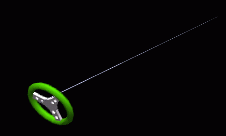
\includegraphics[scale=0.5]{cover/pict/drive} 
\endlatexonly
\html{\htmladdimg[ALIGN=TOP]{pict/drive.png}}

In DRIVE mode the whole scene (besides the coordinate axis and the pinboard) 
is moved as if the user drives in the scene. 
The default button label is "drive" and
the default button location is in the "Navigation" submenu. 
The button belongs to the button group "Navigation".
The DRIVE mode is indicated with a driving wheel as 3D icon.


\subsubsection{COLLIDE}
With COLLIDE collision detection between the viewer and the scene
is enabled/disabled.
The default button label is "collide" and
the default button location is in the "Navigation" submenu. 
The button is a toggle button. The default state is OFF.


\subsubsection{SPEED}
With SPEED you can adjust a scale factor for the velocity in fly, drive
or walk mode.
The default button label is "speed" and
the default button location is in the "Navigation" submenu. 
The button is a slider button. The default minimum speed is 1 and 
the default amximum speed is 30. The default value is 1.
The minimum and maximum and the initial value can be defined in the scope
COVERConfig:
\begin{samepage}
\begin{verbatim}
COVERConfig
{
    ...
    SPEED               <min> <max> <initial value>
    ...
}
\end{verbatim}
\end{samepage}

\subsubsection{Viewpoints}

The "viewpoints" submenu is described in the section about plugins.

\subsection{View Options}

\subsubsection{COORD\_AXIS}
With COORD\_AXIS drawing of a coordinate axis system is enabls/disabled. 
The default button label is "coord axis" and
the default button location is in the "view options" submenu. 
The button is a toggle button. The default state is OFF.

The axis are drawn as lines with a small arrow at the end. The origin
is in the world coordinate origin and the length of the axis is
0.5 * SZENE\_SIZE. The wolrd coordinate system origin is defined
in the scope ScreenConfig (see ection Display Configuration) through
the position of the screen center and the orientation of the screen. 

Typically the x axis points to the right and is drawn red, the
y axis points into the screen and is drawn green and the z axis points
up and is drawn in blue.

\subsubsection{SPECULAR}
With SPECULAR the properties of the light are changed so that objects with
a specular material appear specular.
The default button label is "specular" and
the default button location is in the "view options" submenu. 
The button is a toggle button. The default state is ON.

 
\subsubsection{SPOTLIGHT}
With SPOTLIGHT a lamp like light is attached to the users hand.
The default button label is "spotlight" and
the default button location is in the "view options" submenu. 
The button is a toggle button. The default state is OFF.
		
\subsubsection{STEREO\_SEP}
With STEREO\_SEP the offset between the left and right eye can be set
to zero.
The default button label is "stereo separation" and
the default button location is in the "view options" submenu. 
The button is a toggle button. The default state is OFF.

When STEREO\_SEP switched on, only the ofset is set to zero. The video
mode is not changed to a mono mode, so you don't have any rendering
performance advantage. Use STEREO\_SEP for example if you want to take
pictures or a video from the VE.	

\subsection{Part Manipulation}

\subsubsection{SNAP}
With SNAP constarints for the manipulation of objects are enabled/disabled.
The default button label is "snap" and
the default button location is in the "part manipulation" submenu. 
SNAP is a TOGGLE button. The default state is OFF.

Currently only the cuttingsurface and cutgeometry interaction
supports snapping. In CuttingSurface and CutGeometry 
interaction the plane orientation
is corrected to angles which are multiples of 45 degree.
 
\subsubsection{REMOVE}
In REMOVE mode objects can be selected with the pointer ray and can
removed on button press.

The default button label is "remove" and
the default button location is in the "part manipulation" submenu. 
The button belongs to the button group "Navigation".
The REMOVE mode indicated with a red pointer ray.
 
\subsubsection{UNDO}
With UNDO the REMOVE actions are undone.
The default button label is "undo" and
the default button location is in the "part manipulation" submenu. 
UNDO is a function button. To undo several remove actions, press UNDO
several times.

\subsubsection{MOVE\_PARTS}

With MOVE\_PARTS a cetrtain object can be selected and re-position/re-oriented.
The default button label is "move parts" and
the default button location is in the "part manipulation" submenu. 
The button belongs to the button group "Navigation".
In MOVE\_PARTS mode the object which is closest to the pointer ray is selected
and if the button on the 3D input device is pressed, moved with the
hand. The movement is relatively to the position where the button is pressed.
 


\subsection{Animation}
		
\subsubsection{FORWARD}

FORWARD sets the animation mode to forward playing. This means that
the objects in the animation sequence are drawn one after each other. After the
last object in the sequence it re-starts with the first object. The button appears 
only if COVER receives a COVISE set objects with timesteps.
The default button label is "forward" and
the default button location is in the "animation" submenu.  
FORWARD is a function button.


\subsubsection{Backward}
BACKWARD sets the animation mode to backward playing. This means that
the objects in the animation sequence are drawn in backwards order. After the
first object in the sequence it re-starts with the last object.
The button appears 
only if COVER receives a COVISE set objects with timesteps.
The default button label is "forward" and
the default button location is in the "animation" submenu.  
FORWARD is a function button.

\subsubsection{ANIM\_SPEED}
With ANIM\_SPEED the time interval how long an object in the sequence
is drawn, can be set.
The default button label is "anim speed" and
the default button location is in the "animation" submenu.  
FORWARD is a slider button. The minimum and maximum value and the initial
value can be defind in the scope COVERConfig:

\begin{samepage}
\begin{verbatim}
COVERConfig
{
    ...
    ANIM_SPEED               <min> <max> <initial value>
    ...
}
\end{verbatim}
\end{samepage}

The default values are min=0, max=5,0 and value=1.0.

When the slider is set to the maximum value, objects are drawn as
fast as possible. In this case a timestep containing only a few objects is drawn
faster than a timestep containing a large number of objects.


\subsubsection{Steady Cam}
With STEADY\_CAM the user can attach the viewer to an animated object and
move with this object. For example if the viewer wants to see a car crash
from the view of the person sitting in the car he can attach the camera
to the seat and then he is moved with the crashing car.
The default button label is "steady cam" and
the default button location is in the "animation" submenu.
The button belongs to the button group "Navigation".
		
		
\subsection{COVISE}

The Mapeditor function "Execute" and the parameters of the most important 
COVISE modules can be accessed from within COVER.

\subsubsection{EXECUTE}
With the function button EXECUTE the whole pipeline is eceuted once.
The default button label is "execute pipeline" and
the default button location is in the "COVISE" submenu.
		
\subsubsection{CUTTINGSURFACE}
The module CuttingSurface cuts a plane/cylinder or sphere out of a 
3D grid and interpolates the data to the plane/sphere/cylinder.
The position and orientation of the cutting surface is specified with the
parameters vertex and scalar. In the 2D interface the user has to provide
the orientation of the plane with the parameter vertex (which is the normal
on the plane) and the parameter scalar (which defines the distance from the
origin).

In COVER the user selects the button Cuttingsurface\_i, where i stands for
the instance of the module. A transparent plane is now attached to
the users hand. The plane can be positioned in the scene inside the geometry
by moving the hand to the desired position/orientation. When the Select-button
of the 3D input device is pressed, the current position/orientation is converted
to a normal and distance and sent back to the CuttingSurface module. The
CuttingSurface module is automatically executed and within a few seconds
the new cuttingsurface appears in COVER.

The default button label is "CuttingSurface i", where i is replaced
by the module instance and
the default button location is in the "COVISE" submenu.
The button belongs to the button group "Navigation", this means that if the
previos mode was a navigation mode like XFORM, this mode is switched off. 

\subsubsection{CUTGEOMETRY}
The module CutGeometry cuts a COVISE geometry with a plane.
The position and orientation of the cutting plane is specified with the
parameters vertex and scalar. In the 2D interface the user has to provide
the orientation of the plane with the parameter vertex (which is the normal
on the plane) and the parameter scalar (which defines the distance from the
origin).

In COVER the user selects the button "CutGeometry i", where i stands for
the instance of the module. A transparent plane is now attached to
the users hand. The plane can be positioned in the scene inside the geometry
by moving the hand to the desired position/orientation. When the Select-button
of the 3D input device is pressed, the current position/orientation is converted
to a normal and distance in object space and sent back to the CutGeometry module. 
The CutGeometry module is automatically executed and within a few seconds
the new cutted geometry appears in COVER.

The default button label is "CutGeometry i", where i is replaced
by the module instance and
the default button location is in the "COVISE" submenu.
The button belongs to the button group "Navigation". 
		
\subsubsection{ISOSURFACEP}
The module IsosurfaceP computes an isosurface which contains a
certain point. This point is specified with the parameter point. Then the
value at this point is computed and the all grid points, containings this
value are computed. In the 2D interface the user nters the x, y, and z coordinate
of the point in object coordinates.

In COVER the user selects "IsosurafceP i", where i stands for the instance
of the module. A red sphere is attached to the users hand. The sphere can be 
positioned in the scene by moving the hand to the desired point. 
When the Select-button
of the 3D input device is pressed, the current position is converted
to a object coordinates and sent back to the IsosurfaceP module. The
IsosurfaceP module is automatically executed and within a few seconds
the new isosurface appears in COVER.

The default button label is "IsosurfaceP i", where i is replaced
by the module instance and
the default button location is in the "COVISE" submenu.
The button belongs to the button group "Navigation". 
		
\subsubsection{Tracer}

The COVISE modules TracerUSG, MagTracer, MagBlockTracer, STracer, BlockSTracer,
CellTracer and TetraTrace all computes streamlines or particle traces.

The traces start either on a line or on a plane. In the COVISE module the
line is specified with the parameters startpoint1 and startpoint2, and the
number of traces started on that line is defined with the parameter
no\_startpoints. The plane is specified with the parameters startpoint1,
startpoint2 and normal. 
% Aber wie ?

In COVER the user selects "*Trace* i" from the Pinboard, where *Trace* stand 
for the Tracer module and i for the instance of the module. A red sphere
is now attached to the users hand. When the user presses the select-button
of the 3D input device, the current position is converted to object space
and is taken as startpoint1. The user
can move the hand now to the endpoint of the line while keeping the select-button
pressed. When he releases the button the current position is converted to object
space and is taken as startpoint2. The parameters are sent back to the tracer
module and the module is executed. Within a few seconds the new particle traces
appear in COVER.



\section{Plug Ins}
\label{Plug_Ins}


COVER provides an interface for programming Plug Ins. For details see COVISE Programming Guide,
section COVER Plugin Programming. Below you get a description of some plug ins you may find useful for
your current work.

\subsection{Probe}

{\bf Probe} is a new plugin for 2D probing. To use Probe, select first the Probe button from
the menu; a red icon will appear. If the pointer intersects a 2D object (polygon or 
triangle strips) and the button is pressed, a label will show the coordinates of the 
intersection (relative to the object) plus scalar and vector data values at that point.
The plugin reads the PROBE2D attribute(s) of the grid object which indicate the 
name(s) of the data object(s). You can configure line length and text font of the 
label, the format of the text, and a default for the kind of data to be displayed,
e.g. TEMP, in covise.config, section VRProbe:
\begin{verbatim}
VRProbe
{
   LabelLineLen 90
   LabelFontSize 7
   ScalarFormat %s= %.3f
   VectorFormat %s= %.3f  %.3f %.3f
   DefaultSpecies TEMP (e.g. - if not specified: Unknown)
}
\end{verbatim}
Additional information:
\begin{itemize}
\item don't write anything into the PROBE2D attribute
\item add the following line in the section COVERConfig 
\begin{verbatim}
             MODULE      VRProbe
\end{verbatim}
\end{itemize}
The label will be shown until a new intersection will be selected or the
Probe button will be unselected.

\subsection{Viewpoints}

A viewpoint defines the current position, orientation and scaling factor of the
scene. 
The {\bf Viewpoints} plugin allows to the user to load viewpoints from file
and save them to file ot interactively define new viewpoints. It offers a flight
through all viewpoints or activated only one selected viewpoint. 

The Viewpoint Plugin is activated if the line  
\begin{verbatim}
MODULE VRViewpoint
\end{verbatim}
in COVERConfig (as for all plugins) is available.

\subsubsection{Viewpoint Definition}

Default viewpoints can be defined in covise.config in
the section VRViewpoints, and they will be automatically inserted into the
list of viewpoints:

\begin{verbatim}
VRViewpoints
{
    1    S=1    X = 0 y=0 z=0 h=0 p=0 r=0
    10   S=10   X = 0 y=0 z=0 h=0 p=0 r=0
    100  S=100  X = 0 y=0 z=0 h=0 p=0 r=0
    1000 S=1000 X = 0 y=0 z=0 h=0 p=0 r=0
}
\end{verbatim}

In addition, and even if there is no "Viewpoints" entry in covise.config, there
is a parameter "Viewpoints" in COVER, which contains the name of a custom file
where the viewpoints are stored. If no name is indicated then the file
default.vwp will be loaded (if default.vwp doesn't exist it will be
created).
If a file is specified it will be loaded, and if it doesn't
exist, it will be created.

If COVER is started from the console, the custom viewpoints will be loaded
using  the "-v" option and the path of the .vwp file:
\begin{verbatim}
cover -v example.vwp 
\end{verbatim}


\subsubsection{The Viewpoints Menu}

The button "Viewpoints" opens a submenu with the following entries:
\begin {itemize}
\item "SaveViewPoint"
\item "Flying mode" - toggles animated flight from current to next viewpoint
\item "Flight" - opens a submenu
\item "StartRecord" - starts recording viewpoints
\item "StopRecord" - stops recording viewpoints
\item "First default viewpoint from covise.config" - if one exists
\item   ....
\item "Last viewpoint from covise.config"
\item "First viewpoint from custom viewpoint file" - if one exists
\item  ...
\item "Last viewpoint from custom viewpoint file"
\end {itemize}
By pressing "SaveViewPoint" a new entry, "NewViewpoint", will appear, and
it will be saved in the file. The name "NewViewoints" can be changed in the
file with a text editor.
By chosing a viewpoint and pressing on this entry the viewpoint will be
activated. 

If "flying mode" is active then an animated flight from the
current viewpoint to the selected viewpoint will be started. The selection of viewpoints
can also be done using the keys F1-F12.

The "Flight" button opens a submenu with a list of all viewpoints and
a button "Run". "Run" starts an automatic flight through all selected 
viewpoints in the list. Viewpoints can be removed from the flight by deselecting them 
in the list.

"StartRecord" starts recording viewoints. The viewpoints are saved in vrml
format to a file named animation.wrl. "StopRecord" stops recording viewpoints.
The recorded viewpoints have to be added to a vrml file and become available
in the submenu VrmlViewpoints, as soon as the file is loaded.

\subsection{Snapshot}

This plugin is available when an entry
\begin{verbatim}
MODULE Snapshot
\end{verbatim}
in COVERConfig is present.

When pressing the Snapshot button of the pinboard,
a submenu appears, which has a single button as long
as you have creted no snapshots. When you press this button,
the submenu disappears, and a snapshot will be creted whenever
you press the pointer again. A snapshot may encompass several rgb
files. One or two files are generated for each screen in a screen 
selection list.
By default this list reduces to screen in the first entry in the
ChannelConfig section of covise.config. You may create your own list
by adding a SNAPHOT\_SCREEN entry in section {\sl Snapshot}
of covise.config.

The rgb snapshot files are created by default in the working
directory. You may override this behaviour if a SNAPHOT\_DIR
entry in section {\sl Snapshot} is present, for instance:
\begin{verbatim}
Snapshot
{
SNAPHOT_SCREEN FRONT TOP.
SNAPHOT_DIR /usr/tmp
}
\end{verbatim}

The generated files have the following structure:\newline
snap\{number\}\_\{extra digits\}\_\{left$\mid $right\}Eye\_Screen\{Screen name\}.rgb.
The first number is a snapshot counter. The extra digits have no special
meaning, they are only used in order to prevent new file or button
names from being repeated. Whenever you create a snapshot, a new
viewpoint entry is also created for the Viewpoint plugin, which
should also be in use, otherwise the COVER will crash.
For these new viewpoints associated with snapshot actions,
new buttons are also created in the Snapshot submenu, with
the same name as in the Viewpoint submenu. These names
have the structure: snap\{number\}\_\{extra digits\}.

\subsection{Sketches}

You create drawings in 3D space using this plugin. A sketch is a set of lines.
A line is defined in this context to be a series of connected points.

The Sketches Plugin is activated if the line  
\begin{verbatim}
MODULE Sketcher
\end{verbatim}
in COVERConfig is present.

%\subsubsection{Sketch Generation}

In order to create a sketch, you should activate the {\sl Draw} button
in the {\sl Sketches} menu. Then you may create lines by pressing the
pointer and moving it. When it is released, the current line is finished.
You may create several lines by repeating this operation. When you
are done with one sketch, then you will want to create a new entry
in the list of available sketches. You should press the button {\sl NewSketch}
in this case. But this is not enough to save the sketch in a file
(see below comment on button {\sl SaveSketches}).

The available sketches may be shown or hidden by activating
or deactivating the corresponding entry in the menu.

All sketches are saved to the file specified by 
the COVER parameter {\sl Viewpoints} when you press the button
{\sl SaveSketches}, whose action will be eventually preceded
by the action of button {\sl NewSketch}. 
You may edit this file in order to change
some attributes of the sketches or their lines: sketch name,
color attributes, etc.

The position of the sketching tool with respect to the hand may
be parametrised by a pertinent section in covise.config:
\begin{verbatim}
Sketcher{
ANGLE 5.0
DISPLACEMENT 0.5
SCALE 100.0
}
\end{verbatim}
where SCALE determines the size of the sketching tool,
DISPLACEMENT stands for a displacement along the local Y axis
relative to the sketching-tool size,
and ANGLE parametrises a rotation around the local X axis in degrees.

By way of summary, you may read the table below with explanation to the
buttons in the submenu {\sl Sketches}.
%\subsubsection{The Sketches Menu}
The button {\sl Sketches...} opens a submenu with the following entries:
\begin {itemize}
\item "Draw" - enters drawing mode
\item "NewSketch" - ends the definition of a sketch and creates a new entry in the list of sketches
\item "SaveSketch" - saves all sketches to file
\item "First sketch name" - if one exists
\item "Second sketch name" - if one exists
\item   \ldots
\end {itemize}


